% ============================================================
% REPORTE DE INVESTIGACION --- DatosAbiertos2026-v3
% Gobernanza y Calidad de Datos en Portales de Gobierno Abierto:
% Una Evaluacion Cuantitativa del Caso Nuevo Leon 2026
% Formato: LaTeX / APA 7 --- biblatex + biber
% ============================================================
\documentclass[12pt,letterpaper]{article}

% -- Paquetes --------------------------------------------------
\usepackage[utf8]{inputenc}
\usepackage[T1]{fontenc}
\usepackage[spanish,es-tabla]{babel}
\usepackage{mathptmx}
\usepackage[left=2.5cm,right=2.5cm,top=2.5cm,bottom=2.5cm]{geometry}
\usepackage{setspace}\doublespacing
\usepackage{parskip}
\usepackage{titlesec}
\usepackage{booktabs}
\usepackage{longtable}
\usepackage{array}
\usepackage{graphicx}
\usepackage{caption}
\usepackage{amsmath}
\usepackage{hyperref}
\usepackage[style=apa,backend=biber,language=spanish]{biblatex}
\usepackage{csquotes}

% -- Configuracion APA ----------------------------------------
\titleformat{\section}{\normalfont\bfseries\large}{\thesection.}{0.5em}{}
\titleformat{\subsection}{\normalfont\bfseries}{\thesubsection.}{0.5em}{}
\titleformat{\subsubsection}{\normalfont\itshape}{\thesubsubsection.}{0.5em}{}

\hypersetup{colorlinks=true,linkcolor=black,citecolor=black,urlcolor=blue}

\addbibresource{referencias.bib}

\begin{document}

% ============================================================
% PORTADA
% ============================================================
\begin{titlepage}
\centering\vspace*{2cm}

{\Large\bfseries Universidad Aut\'onoma de Nuevo Le\'on}\\[0.3cm]
{\large Facultad de Filosof\'ia y Letras}\\[0.3cm]
{\large Gesti\'on de la Informaci\'on y Recursos Digitales}\\[2cm]

{\LARGE\bfseries Gobernanza y Calidad de Datos en Portales de Gobierno Abierto: Una Evaluaci\'on Cuantitativa del Caso Nuevo Le\'on 2026}\\[2cm]

{\large\bfseries Reporte de Investigaci\'on --- Metodolog\'ia Cuantitativa}\\[1.5cm]

{\large Elaborado por:}\\[0.3cm]
{\large Aldo Giovanni Mart\'inez Pineda}\\[1.5cm]

{\large Monterrey, Nuevo Le\'on, M\'exico}\\[0.3cm]
{\large Mayo de 2026}

\vfill
\end{titlepage}

% -- INDICE ---------------------------------------------------
\tableofcontents
\newpage

% ============================================================
% RESUMEN
% ============================================================
\begin{abstract}
\noindent
Este reporte presenta los resultados de una evaluaci\'on cuantitativa y automatizada
de la calidad de los datos publicados en el portal de datos abiertos del Gobierno del
Estado de Nuevo Le\'on (\texttt{catalogodatos.nl.gob.mx}). El estudio utiliz\'o un
\textit{pipeline} computacional desarrollado en Python~3.13 para evaluar \textbf{288
recursos} de datos distribuidos en 19 categor\'ias tem\'aticas, aplicando el marco de
calidad establecido por el est\'andar internacional ISO/IEC 25012:2008 en siete
dimensiones: completitud, exactitud, consistencia, unicidad, puntualidad,
documentaci\'on y apertura. Los resultados muestran que el portal obtuvo un score
global promedio de \textbf{88.83 puntos sobre 100}, con el 65.6\,\% de los recursos
clasificados en el nivel Gold ($\geq 90$ puntos). La dimensi\'on de completitud
present\'o la mayor variabilidad ($\sigma = 24.47$), lo que indica oportunidades de
mejora en la captura de datos por parte de las dependencias publicadoras. El estudio
establece una l\'inea base metodol\'ogica que puede extenderse a otros portales de
gobierno abierto en M\'exico.

\vspace{0.5cm}
\noindent\textbf{Palabras clave:} calidad de datos, gobierno abierto, ISO/IEC 25012,
DAMA-DMBOK, Nuevo Le\'on, \textit{pipeline} ETL, datos abiertos.
\end{abstract}

\newpage

% ============================================================
% 1. INTRODUCCION
% ============================================================
\section{Introducci\'on}

La publicaci\'on de datos gubernamentales en formatos abiertos constituye un
mecanismo central de la transparencia p\'ublica, seg\'un lo establece la Ley General
de Transparencia y Acceso a la Informaci\'on P\'ublica \parencite{lgtaip2015}.
No obstante, publicar datos no equivale a publicar datos de calidad. Para que
la informaci\'on abierta sea \textit{apta para su uso} ---en el sentido propuesto
por \textcite{wang1996}---, cada recurso debe satisfacer criterios verificables
de completitud, exactitud, consistencia y documentaci\'on.

El portal \texttt{catalogodatos.nl.gob.mx} del Gobierno del Estado de Nuevo Le\'on
funciona sobre la plataforma CKAN (\textit{Comprehensive Knowledge Archive
Network}), empleada por gobiernos de m\'as de 50 pa\'ises para gestionar sus
cat\'alogos de datos \parencite{neumaier2016}. A trav\'es de este portal, las
dependencias estatales distribuyen conjuntos de datos en formatos como CSV, JSON
y XLSX. Sin embargo, la ausencia de validaciones previas a la carga permite que
recursos con deficiencias graves convivan con recursos de alta calidad.

Este reporte documenta la evaluaci\'on cuantitativa de los datos disponibles en
el portal, utilizando un instrumento de medici\'on automatizado alineado al
est\'andar ISO/IEC 25012:2008 \parencite{iso25012}, al cuerpo de conocimiento
profesional DAMA-DMBOK \parencite{dama2017}, y al marco de evaluaci\'on de
\textcite{vetro2016} para portales de gobierno abierto. El c\'odigo fuente del
proyecto (\textit{DatosAbiertos2026-v3}) es p\'ublico y permite la replicaci\'on
completa del an\'alisis.

% ============================================================
% 2. PREGUNTAS DE INVESTIGACION E HIPOTESIS
% ============================================================
\section{Objetivos}

\subsection{Objetivo general}

Evaluar de forma cuantitativa la calidad de los datos abiertos publicados en el
portal del Gobierno del Estado de Nuevo Le\'on, mediante un instrumento
automatizado alineado a los est\'andares ISO/IEC 25012:2008, ISO~8000 y DAMA-DMBOK.

\subsection{Objetivos espec\'ificos}

\begin{enumerate}
  \item Implementar un \textit{pipeline} computacional que eval\'ue siete
    dimensiones de calidad de datos: completitud, exactitud, consistencia,
    unicidad, puntualidad, documentaci\'on y apertura.
  \item Aplicar el instrumento a la totalidad de los recursos disponibles en
    el portal (muestreo censal).
  \item Clasificar los recursos seg\'un niveles de salud de datos (Gold,
    Silver, Bronze) e identificar las dimensiones con puntajes deficientes.
  \item Comparar los resultados con la evaluaci\'on previa realizada por
    \textcite{alanis2024} en 2024.
\end{enumerate}

% ============================================================
% 3. PREGUNTAS E HIPOTESIS
% ============================================================
\section{Preguntas de investigaci\'on e hip\'otesis}

El estudio busc\'o responder cuatro preguntas:

\begin{enumerate}
  \item \textquestiondown Cu\'al es el nivel de calidad promedio de los datos
    publicados en el portal, medido con el \textit{framework} ISO/IEC 25012?
  \item \textquestiondown Cu\'al es la distribuci\'on de los recursos seg\'un
    los niveles Gold, Silver y Bronze?
  \item \textquestiondown Cu\'ales son las dimensiones con mayor y menor
    desempe\~no en el cat\'alogo?
  \item \textquestiondown Existen diferencias observables en la calidad de
    datos entre las dependencias publicadoras?
\end{enumerate}

El protocolo de investigaci\'on formul\'o cuatro hip\'otesis (H\textsubscript{1} a
H\textsubscript{4}). Este reporte contrasta directamente dos de ellas:

\begin{itemize}
  \item \textbf{H\textsubscript{1}:} El score global promedio se ubica por
    debajo de 90 puntos sobre 100.
  \item \textbf{H\textsubscript{4}:} M\'as del 60\,\% de los recursos
    alcanzan el nivel Gold ($\geq 90$ puntos).
\end{itemize}

\noindent Las hip\'otesis H\textsubscript{2} (diferencia estad\'istica entre
dependencias mediante ANOVA) y H\textsubscript{3} (completitud como dimensi\'on
de mayor peso relativo en el score) no se contrastaron con pruebas inferenciales
en esta fase del estudio. H\textsubscript{2} requiere verificar supuestos de
normalidad y homogeneidad de varianza que no se ejecutaron; H\textsubscript{3}
se aborda descriptivamente en la secci\'on de resultados (la completitud, con
peso del 30\,\%, present\'o una media de 85.09, inferior a la media ponderada
global, lo que confirma su influencia negativa en el score final).

% ============================================================
% 3. MARCO METODOLOGICO
% ============================================================
\section{Marco metodol\'ogico}

El estudio adopt\'o un dise\~no \textbf{descriptivo, transversal y no
experimental}. Descriptivo porque busca medir y reportar el estado actual de
la calidad de datos del portal sin manipular variables. Transversal porque la
recoleccion se realiz\'o en un solo momento temporal. No experimental porque
no se asignaron tratamientos ni se controlaron condiciones.

\subsection{Fundamentos normativos}

La evaluaci\'on se sustenta en tres marcos de referencia internacionales. El primero es
el est\'andar \textbf{ISO/IEC 25012:2008}, que establece un modelo de calidad de datos
compuesto por 15 caracter\'isticas organizadas en dos categor\'ias: calidad inherente
(independiente del sistema) y calidad dependiente del sistema \parencite{iso25012}.
Para este estudio se seleccionaron siete de estas caracter\'isticas: completitud,
exactitud, consistencia, unicidad, actualidad (denominada aqu\'i puntualidad),
comprensibilidad (denominada documentaci\'on) y accesibilidad (denominada apertura).

El segundo marco es el \textbf{DAMA-DMBOK} \parencite{dama2017}, que define las
mejores pr\'acticas para la gesti\'on de datos a nivel organizacional. Este marco orienta
la evaluaci\'on de los metadatos de gobernanza: la presencia de campos como autor,
mantenedor, licencia, frecuencia de actualizaci\'on y descripci\'on del \textit{dataset}.

El tercer referente es el \textbf{Open Data Quality Measurement Framework} de
\textcite{vetro2016}, que aport\'o la l\'ogica de clasificaci\'on de recursos en tres
niveles de salud de datos (Gold, Silver, Bronze), adaptados al contexto del portal de
Nuevo Le\'on.

\subsection{Dise\~no del instrumento: el pipeline ETL}

El instrumento de medici\'on es un \textit{pipeline} computacional automatizado
desarrollado en Python~3.13, que opera como un sistema de Extracci\'on, Transformaci\'on
y Carga (ETL). Su arquitectura se divide en tres m\'odulos:

\begin{enumerate}
  \item \textbf{M\'odulo Extractor} (\texttt{pipeline/extractor.py},
    \texttt{pipeline/fetcher.py}): Se conecta al API REST del portal CKAN para
    descubrir todos los \textit{datasets} y recursos disponibles, y descarga cada
    archivo para su an\'alisis.
  \item \textbf{M\'odulo Evaluador} (\texttt{quality\_scorer.py}): Calcula las siete
    dimensiones de calidad para cada recurso. Las dimensiones de contenido operan
    sobre el DataFrame de Pandas descargado; las de cat\'alogo (puntualidad,
    documentaci\'on, apertura) operan sobre los metadatos CKAN.
  \item \textbf{M\'odulo de Persistencia} (\texttt{pipeline/persistence.py}): Almacena
    los resultados en CSV, JSON y Parquet para su an\'alisis posterior.
\end{enumerate}

La \textbf{validez de contenido} del instrumento se sustenta en la
correspondencia directa entre las siete dimensiones evaluadas y las
caracter\'isticas del modelo ISO/IEC 25012:2008 \parencite{iso25012}. Los
pesos asignados a cada dimensi\'on (completitud 30\,\%, exactitud 25\,\%,
consistencia 15\,\%) reproducen la jerarqu\'ia documentada en el DAMA-DMBOK
\parencite{dama2017}. La \textbf{confiabilidad} es inherente a la naturaleza
algor\'itmica del instrumento: ante la misma entrada, produce los mismos
resultados en cada ejecuci\'on, lo que garantiza la reproducibilidad del
estudio \parencite{vizcaino2023}.

\subsection{Operacionalizaci\'on de las dimensiones}

La Tabla~\ref{tab:operacionalizacion} describe c\'omo se calcula cada dimensi\'on en el
c\'odigo, tomando como referencia el m\'odulo \texttt{quality\_scorer.py}.

\begin{table}[h!]
\centering
\caption{Operacionalizaci\'on de las dimensiones de calidad}
\label{tab:operacionalizacion}
\begin{tabular}{p{2.6cm}p{8cm}p{1.8cm}}
\toprule
\textbf{Dimensi\'on} & \textbf{F\'ormula implementada} & \textbf{Peso} \\
\midrule
Completitud &
  $C = \dfrac{\text{celdas no nulas}}{\text{total de celdas}} \times 100$ & 30\,\% \\[10pt]
Exactitud &
  $A = 100 - \dfrac{\text{mixtos}}{n}\times40 - \dfrac{\text{espacios}}{n}\times15
  - \dfrac{\text{constantes}}{n}\times20$ & 25\,\% \\[10pt]
Consistencia &
  Penalizaci\'on por valores at\'ipicos (IQR) e inconsistencias de texto (may\'usculas/espacios) & 15\,\% \\[6pt]
Unicidad &
  $U = 100 - (\%\,\text{duplicados} \times 2)$ & 8\,\% \\[6pt]
Puntualidad &
  Latencia vs.\ frecuencia declarada; interpolaci\'on lineal entre $f$ y $2f$ & 5\,\% \\[6pt]
Documentaci\'on &
  Descripci\'on (30~pts) + recursos descritos (30~pts) + licencia (20~pts) + metodolog\'ia (20~pts) & 10\,\% \\[6pt]
Apertura &
  Formato abierto (40~pts) + licencia abierta (35~pts) + acceso directo (25~pts) & 7\,\% \\
\bottomrule
\end{tabular}
\end{table}

\noindent\textit{Nota.} La suma de pesos es 1.00. El score global se calcula como:
$S = \sum_{i} d_i \times w_i$.

\subsection{Muestra}

Se emple\'o un \textbf{muestreo censal}: se evalu\'o el 100\,\% de los recursos
disponibles con URL de descarga activa y formato parseable (CSV, JSON, XLSX). El
universo final comprendi\'o \textbf{288 recursos} pertenecientes a \textbf{19
categor\'ias tem\'aticas}, publicados por dependencias gubernamentales estatales. Se
excluyeron archivos PDF no tabulares y recursos con URLs inaccesibles al momento
de la evaluaci\'on.

% ============================================================
% 4. RESULTADOS
% ============================================================
\section{Resultados cuantitativos}

\subsection{Desempe\~no global del portal}

La evaluaci\'on arroj\'o un \textbf{score global promedio de 88.83 puntos} (mediana =
91.61; $\sigma$ = 9.48; m\'in.\ = 52.61; m\'ax.\ = 98.23). Esto confirma la hip\'otesis
H\textsubscript{1}: el portal no alcanza el umbral de ``Excelente'' ($\geq 90$
puntos) en promedio, si bien la mediana s\'i lo supera, lo que indica que la
distribuci\'on est\'a sesgada hacia abajo por un conjunto de recursos con baja calidad.

La Figura~\ref{fig:distribucion} muestra la distribuci\'on completa de scores. Se
observa una concentraci\'on principal entre 88 y 98 puntos, y una cola izquierda que
agrupa recursos con deficiencias significativas en completitud o documentaci\'on.

\begin{figure}[h!]
\centering
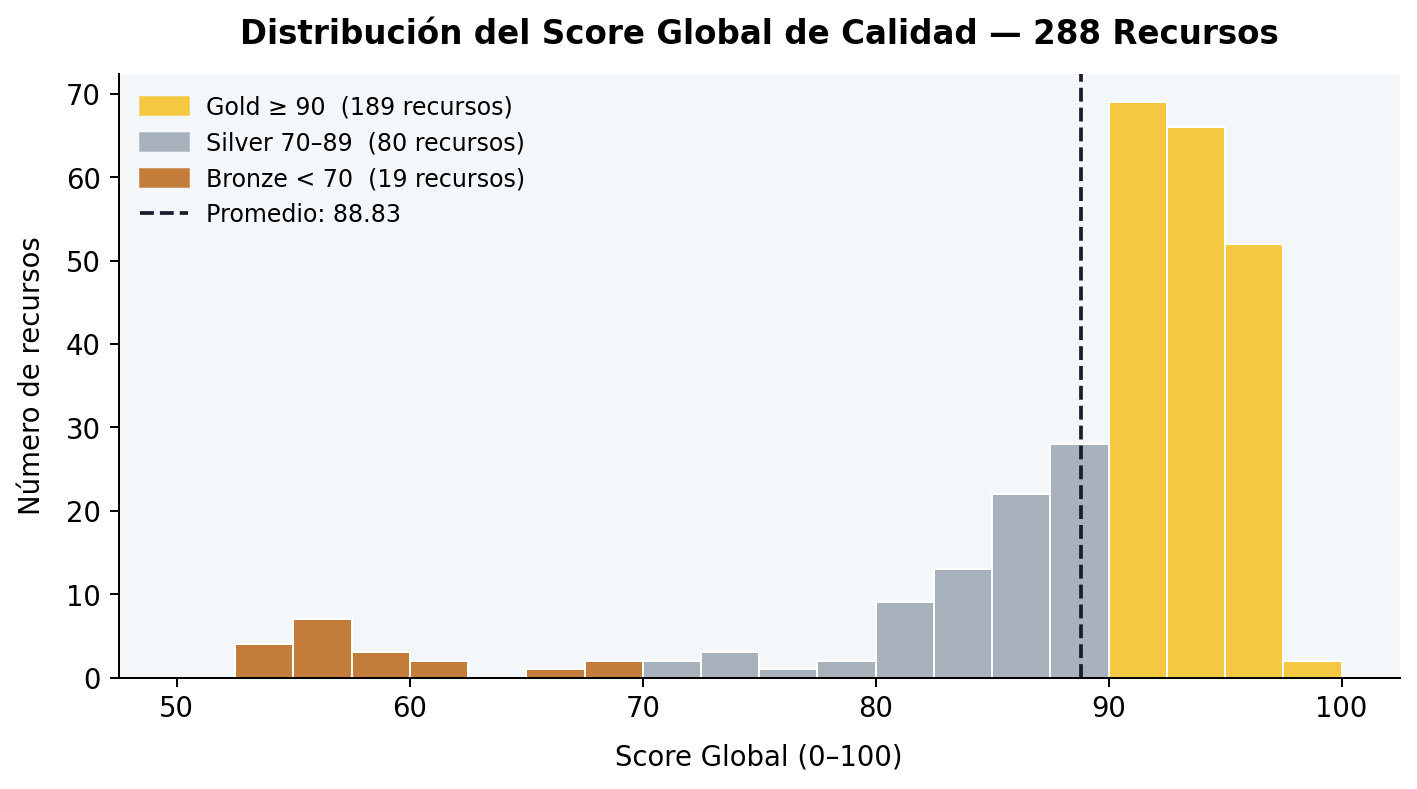
\includegraphics[width=0.9\textwidth]{figures/fig1_distribucion_scores.png}
\caption{Distribuci\'on del score global de calidad para los 288 recursos evaluados.
Las barras est\'an coloreadas seg\'un la clasificaci\'on Medallion: dorado (Gold
$\geq 90$), plateado (Silver 70--89) y bronce (Bronze $< 70$).}
\label{fig:distribucion}
\end{figure}

\subsection{Clasificaci\'on por niveles de salud de datos}

La Figura~\ref{fig:clasificacion} y la Tabla~\ref{tab:clasificacion} presentan la
distribuci\'on de recursos seg\'un la escala de clasificaci\'on adaptada de
\textcite{vetro2016}.

\begin{figure}[h!]
\centering
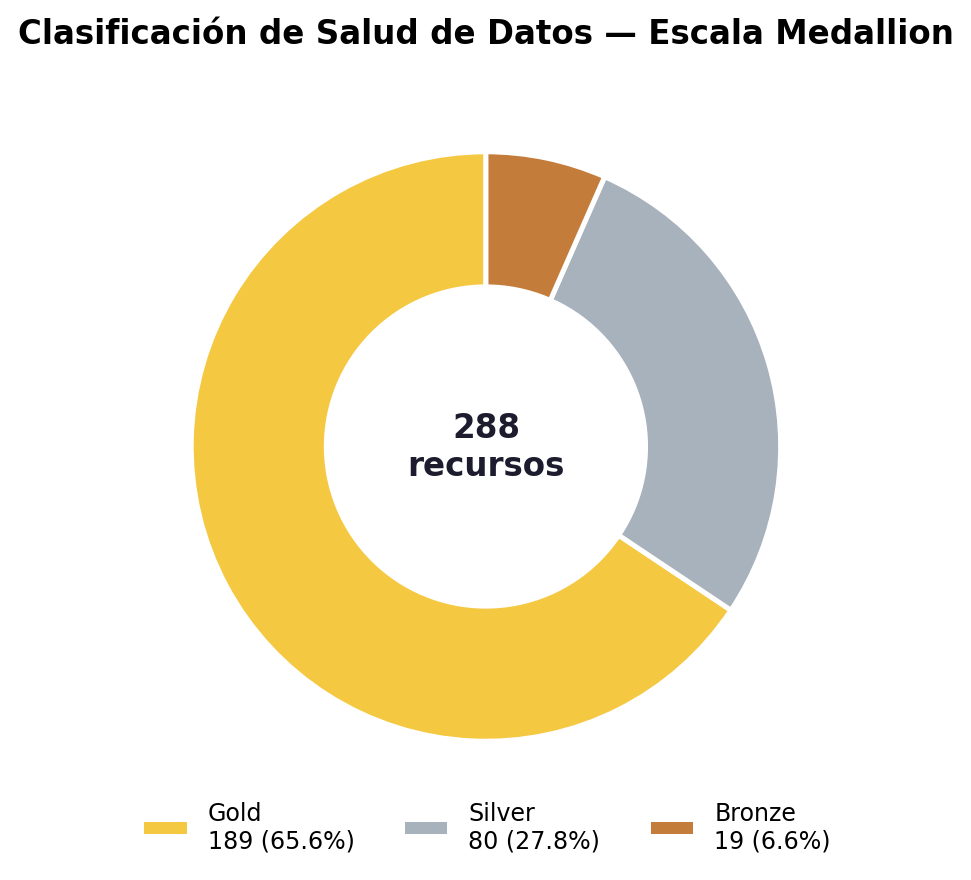
\includegraphics[width=0.62\textwidth]{figures/fig3_clasificacion.png}
\caption{Distribuci\'on de recursos seg\'un la clasificaci\'on Medallion de salud de datos.}
\label{fig:clasificacion}
\end{figure}

\begin{table}[h!]
\centering
\caption{Distribuci\'on de recursos por nivel de calidad}
\label{tab:clasificacion}
\begin{tabular}{lccc}
\toprule
\textbf{Nivel} & \textbf{Umbral} & \textbf{Recursos} & \textbf{Porcentaje} \\
\midrule
Gold   & $\geq 90$ puntos & 189 & 65.6\,\% \\
Silver & 70--89 puntos    & 80  & 27.8\,\% \\
Bronze & $< 70$ puntos    & 19  & 6.6\,\%  \\
\midrule
\textbf{Total} & --- & \textbf{288} & \textbf{100\,\%} \\
\bottomrule
\end{tabular}
\end{table}

El 65.6\,\% de los recursos alcanz\'o el nivel Gold, lo que \textbf{confirma la
hip\'otesis H\textsubscript{4}} (m\'as del 60\,\% en Gold). Sin embargo, el 6.6\,\% de
los recursos en Bronze (19 recursos) representa un pasivo de calidad que requiere
atenci\'on prioritaria por parte de las dependencias responsables.

\subsection{Desempe\~no por dimensi\'on de calidad}

La Tabla~\ref{tab:dimensiones} y la Figura~\ref{fig:dimensiones} presentan el
desempe\~no promedio de cada dimensi\'on.

\begin{table}[h!]
\centering
\caption{Estad\'isticas descriptivas por dimensi\'on de calidad}
\label{tab:dimensiones}
\begin{tabular}{lcccc}
\toprule
\textbf{Dimensi\'on} & \textbf{Peso} & \textbf{Media} & \textbf{Mediana} & \textbf{$\sigma$} \\
\midrule
Completitud    & 30\,\% & 85.09 & 95.65 & 24.47 \\
Exactitud      & 25\,\% & 92.35 & 93.33 &  5.67 \\
Consistencia   & 15\,\% & 95.64 & 96.00 &  8.22 \\
Unicidad       &  8\,\% & 89.76 & 100.00 & 27.23 \\
Puntualidad    &  5\,\% & 95.33 & 96.94 &  3.52 \\
Documentaci\'on & 10\,\% & 72.40 & 72.00 &  6.63 \\
Apertura       &  7\,\% & 95.43 & 100.00 & 12.52 \\
\midrule
\textbf{Score Global} & 100\,\% & \textbf{88.83} & \textbf{91.61} & \textbf{9.48} \\
\bottomrule
\end{tabular}
\end{table}

\begin{figure}[h!]
\centering
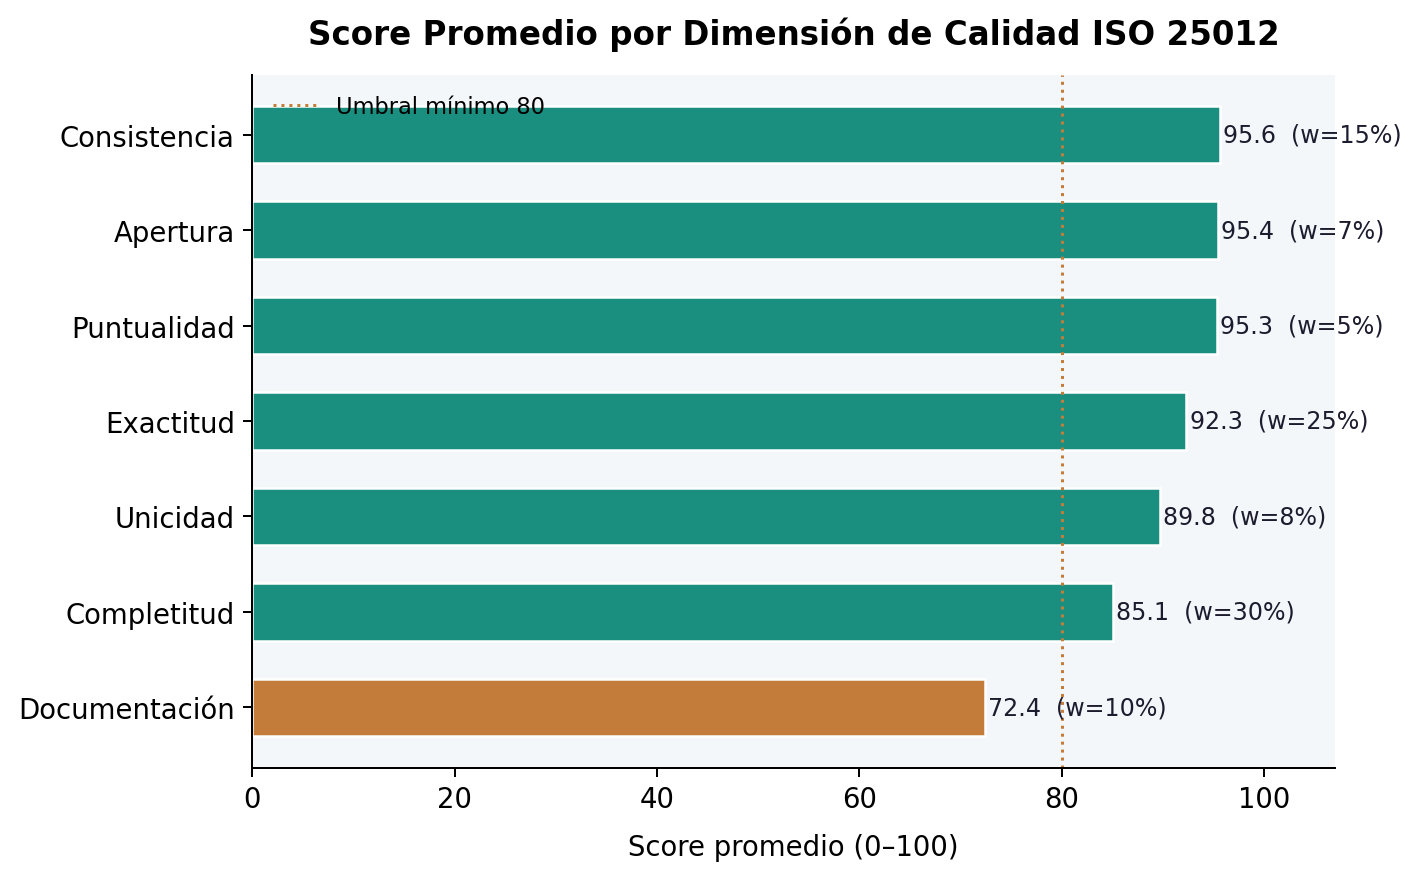
\includegraphics[width=0.9\textwidth]{figures/fig2_dimensiones.png}
\caption{Score promedio por dimensi\'on de calidad ISO~25012. La barra de completitud
aparece destacada por ubicarse por debajo del umbral de referencia de 80 puntos.
Los valores entre par\'entesis indican el peso ponderado de cada dimensi\'on.}
\label{fig:dimensiones}
\end{figure}

Cinco de las siete dimensiones superan los 89 puntos. Las dos dimensiones con
puntajes deficientes son \textbf{completitud} ($\mu = 85.09$) y
\textbf{documentaci\'on} ($\mu = 72.40$). La desviaci\'on est\'andar de la
completitud ($\sigma = 24.47$) es la m\'as alta del conjunto, lo que indica que
algunas dependencias mantienen \textit{datasets} pr\'acticamente completos
mientras que otras registran tasas de valores nulos superiores al 50\,\%.

La dimensi\'on de \textbf{documentaci\'on}, con peso del 10\,\% en el score
global, obtuvo el puntaje m\'as bajo ($\mu = 72.40$). La mayor\'ia de los
\textit{datasets} carecen de descripciones con extensi\'on suficiente,
diccionarios de datos o referencias metodol\'ogicas, lo que dificulta que
investigadores y periodistas puedan reutilizar estos datos sin contactar
directamente a la dependencia publicadora.

\subsection{Desempe\~no por dependencia gubernamental}

La Figura~\ref{fig:organizaciones} muestra las diez dependencias con mayor score
promedio entre las que publicaron dos o m\'as recursos, destacando la Universidad de
Ciencias de la Seguridad (96.20), la Junta Local de Conciliaci\'on y Arbitraje (95.96)
y la Secretar\'ia de Salud (94.14, con la muestra m\'as grande: 29 recursos evaluados).

\begin{figure}[h!]
\centering
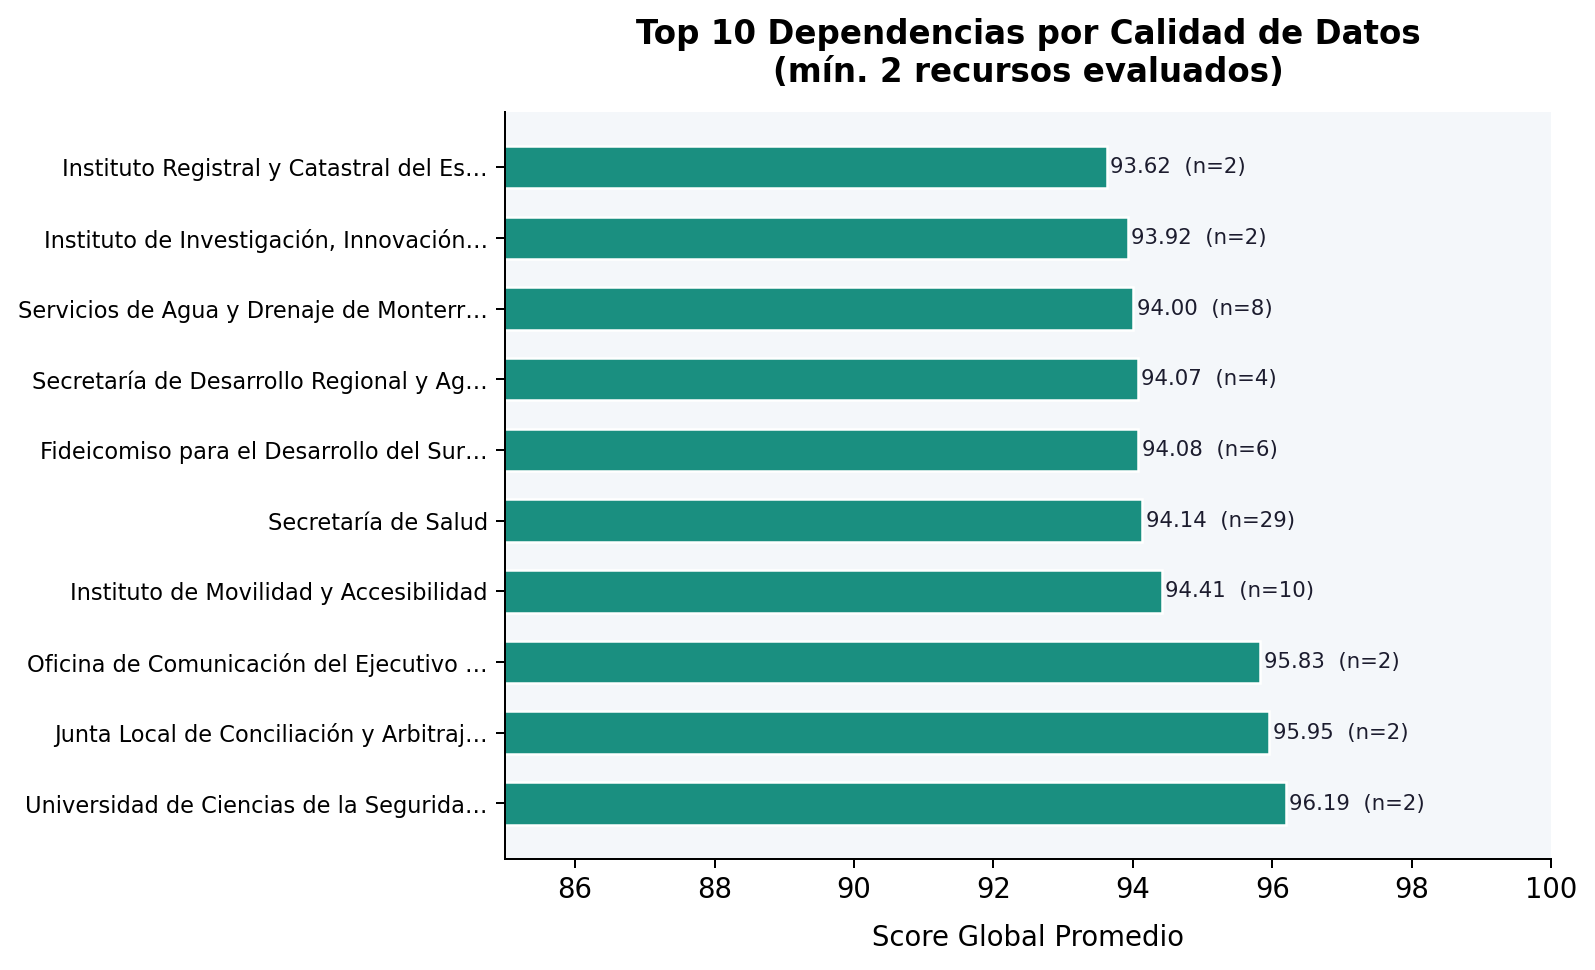
\includegraphics[width=\textwidth]{figures/fig4_top_organizaciones.png}
\caption{Top 10 dependencias gubernamentales por score global promedio de calidad de datos
(m\'inimo 2 recursos evaluados).}
\label{fig:organizaciones}
\end{figure}

% ============================================================
% 5. DISCUSION
% ============================================================
\section{Discusi\'on}

\subsection{Interpretaci\'on de los resultados principales}

Un score promedio de 88.83 puntos posiciona al portal de Nuevo Le\'on como un sistema
de datos abiertos con un nivel de madurez \textit{intermedio-alto} utilizando los
par\'ametros propuestos por \textcite{vetro2016}. Comparado con los portales europeos
analizados en ese estudio, donde la mayor\'ia report\'o puntajes de completitud por
debajo del 70\,\%, el portal de Nuevo Le\'on muestra un desempe\~no relativamente
favorable, aunque con margen de mejora en las dimensiones de contenido.

Que la documentaci\'on sea la dimensi\'on m\'as d\'ebil ($\mu = 72.40$) coincide
con lo reportado por \textcite{neumaier2016} en portales CKAN europeos: la
completitud de metadatos tiende a ser inferior a la calidad t\'ecnica del
contenido tabular. Las dependencias cargan archivos pero no redactan
descripciones ni publican diccionarios de datos, lo que reduce la utilidad
de los recursos para usuarios ajenos a la dependencia.

La dispersi\'on de la completitud ($\sigma = 24.47$) confirma que no existe
un protocolo de validaci\'on uniforme antes de publicar datos en el portal.
Algunas dependencias entregan tablas pr\'acticamente completas; otras dejan
columnas enteras vac\'ias. Implementar una validaci\'on autom\'atica antes de
la carga ---como la que ofrece el propio API de CKAN--- reducir\'ia esta
variabilidad.

\subsection{Contraste con el estudio previo}

El trabajo de \textcite{alanis2024}, que evalu\'o 17 \textit{datasets} del mismo portal
en 2024 utilizando cuatro dimensiones de calidad y herramientas de inteligencia
artificial comercial, sirve como punto de referencia hist\'orico. El presente estudio
ampli\'o el alcance a 288 recursos y siete dimensiones, lo que permite una visi\'on m\'as
completa del estado del cat\'alogo. Mientras que el estudio previo depend\'ia de APIs
comerciales (Perplexity con Llama~3.1 y GPT-4), este trabajo utiliza algoritmos
deterministas que garantizan la reproducibilidad de los resultados.

\subsection{Limitaciones}

El estudio tiene cuatro limitaciones que deben considerarse al interpretar los
resultados. Primera, los recursos en formato PDF (no tabulares) quedaron fuera
del alcance del \textit{pipeline}, por lo que una fracci\'on del cat\'alogo no
fue evaluada. Segunda, la dimensi\'on de puntualidad depende de que las
dependencias declaren correctamente la frecuencia de actualizaci\'on en sus
metadatos CKAN; si este campo est\'a vac\'io o es incorrecto, la evaluaci\'on
pierde precisi\'on. Tercera, el componente de enriquecimiento sem\'antico con
Vertex~AI (Google Gemini 2.5 Flash) no estaba activo durante la evaluaci\'on
por ausencia de credenciales en el entorno, de modo que los scores reportados
corresponden exclusivamente a las evaluaciones algor\'itmicas deterministas.
Cuarta, las hip\'otesis H\textsubscript{2} (ANOVA por dependencia) y
H\textsubscript{3} (peso relativo de la completitud) no se contrastaron con
pruebas inferenciales formales; su verificaci\'on queda pendiente para una
segunda fase del estudio.

\subsection{Trabajo futuro}

Tres l\'ineas de trabajo se derivan directamente de los hallazgos de este
estudio. Primera, ejecutar la evaluaci\'on en un segundo momento temporal
para construir una serie longitudinal y verificar si las dependencias
mejoran sus procesos de publicaci\'on. Segunda, replicar el \textit{pipeline}
en portales de otros estados mexicanos (Jalisco, Ciudad de M\'exico, Yucat\'an)
para generar comparaciones inter-estatales. Tercera, activar el m\'odulo de
enriquecimiento sem\'antico con Vertex~AI y evaluar si las descripciones
generadas por IA mejoran la dimensi\'on de documentaci\'on del cat\'alogo.

% ============================================================
% 6. CONCLUSIONES
% ============================================================
\section{Conclusiones}

Este estudio demuestra que el portal de datos abiertos del Gobierno del Estado de
Nuevo Le\'on mantiene un nivel de calidad promedio de \textbf{88.83/100 puntos}, con
el \textbf{65.6\,\%} de sus recursos clasificados en el nivel Gold, lo que confirma
las hip\'otesis H\textsubscript{1} y H\textsubscript{4} establecidas en el protocolo
de investigaci\'on.

Las principales conclusiones son las siguientes:

\begin{enumerate}
  \item Las dimensiones t\'ecnicas (exactitud: 92.35; consistencia: 95.64;
    apertura: 95.43) superan el umbral de 90 puntos. Las dimensiones de
    completitud (85.09) y documentaci\'on (72.40) presentan puntajes
    deficientes que requieren intervenci\'on directa.
  \item La dispersi\'on de la completitud ($\sigma = 24.47$) confirma que
    no existe un protocolo homog\'eneo de validaci\'on de datos previa a su
    carga en el portal.
  \item El instrumento de medici\'on desarrollado en este proyecto ---basado
    en ISO/IEC 25012 y DAMA-DMBOK--- es determinista, reproducible y de
    c\'odigo abierto. Puede aplicarse a otros portales CKAN en M\'exico
    sin modificaciones.
  \item Se recomienda que la administraci\'on estatal exija a las
    dependencias: descripciones de al menos 120 caracteres, tres o m\'as
    etiquetas tem\'aticas, licencia declarada y frecuencia de actualizaci\'on
    antes de aprobar la carga de nuevos \textit{datasets}.
\end{enumerate}

\noindent Los datos y el c\'odigo de este estudio quedan disponibles en el
repositorio p\'ublico del proyecto para que futuras evaluaciones puedan
verificar si las dependencias mejoran sus pr\'acticas de publicaci\'on.

% ============================================================
% REFERENCIAS
% ============================================================
\printbibliography[title={Referencias}]

\end{document}
